\documentclass[11pt, letterpaper, dvipsnames]{article} % for a4 sized paper, define a4paper instead of letterpaper
\usepackage{multivar-notes}

\begin{document}
\vspace*{\stretch{1}}
\begin{center}\large \textbf{MA662: Multivariable Calculus} \\[12pt]

	\small \textsc{Jiahua Chen}	\\[12pt]
	
	Spring 2019\end{center}
	\vspace{2em}
	
	\begin{changemargin}{.7in}{.7in} 
	These are the course notes for Multivariable Calculus (\textbf{MA662}) at Hotchkiss taught by Dr. Weiss. These notes were last updated \today. Any sections denoted with asterisks \texttt{(***)} are currently incomplete, and I will update them when I get to those. Although the notes are my own documentation, I've appropriated some of Krit's\footnote{Krit's version of these notes are here: \flushright{\scriptsize\texttt{https://drive.google.com/file/d/1nErNuy8LWLYCIXDgkJ2Q5dOtwFVzuoeJ/}}} notes for reference. 
	\end{changemargin}
	
\vspace{\stretch{4}}

\newpage
\tableofcontents

\newpage
% !TEX root = ../multivar-notes.tex
\section{Topology}
\subsection{Subsets of $\R$}
\subsubsection*{January 7, 2019}
We start with an in-depth exploration of topology first in single-dimensional reals.

\begin{defn}{Bounds}
Let $X\subseteq \R$. Then\dots
\begin{enumerate}
	\item $u\in \R$ is called an \ul{upper bound} of $X$ if $x\leq u,\ \forall x\in X$.
	\item $l\in \R$ is called a \ul{lower bound} of $X$ if $x\geq l,\ \forall x\in X$.
\end{enumerate}
\end{defn}

It is an axiomatic property of $\R$ that each subset of $\R$ bounded above has a least upper bound and, likewise, each subset that is bounded below has a greatest lower bound.

\begin{defn}{Extremum}
	Let $X\subseteq \R$ be bounded. Then\dots
	\begin{enumerate}
	\item $y = \Sup(X)$ (\ul{supremum} of X) if $y$ is an upper bound and, $y'$ is another upper bound, then $y' \geq y$.
	\item $z = \Inf(X)$ (\ul{infinum} of X) if $z$ is an lower bound and, $z'$ is another lower bound, then $z' \leq z$.
\end{enumerate}
Also if\dots
\begin{enumerate}
\item $\Sup(X)\in X$, then we call it the maximum of $X$.
\item $\Inf(X)\in X$, then we call it the minimum of $X$.
\end{enumerate}
\end{defn}

\example

$X = (0,1)$ \qquad
$\Sup(X) = 1$ \qquad
$\Inf(X) = 0$ \qquad
no max, no min

$X = [0,1]$ \qquad
$\Sup(X) = \Max(X) = 1$ \qquad
$\Inf(X) = \Min(X) = 0$

\begin{proposition}
	If $X\subseteq \R$, bounded above, then $y = \Sup(X)$ iff
	\begin{enumerate}[(i)]
		\item $y$ is an upper bound
		\item $\forall \epsilon > 0$, $\exists x\in X$ such that $x>y-\epsilon$
	\end{enumerate}
\end{proposition}
\begin{proof}
Let $y = \Sup(X)$. \begin{enumerate}[(i)]
\item is true by definition
\item Suppose $\exists \epsilon > 0$ such that there is no $x\in X$ with $x>y-\epsilon$. \\
Then $x\leq y-\epsilon \forall x\in X$. But that makes $y-\epsilon < y$ a smaller upper bound of $X$, which contradicts $y=\Sup(X)$
\end{enumerate}

Suppose next that (i) and (ii) hold for $y\in \R$. We show that $y = \Sup(X)$. Clearly, y is an upper bound by (i), so let $y'$ be a smaller upper bound for the sake of contradiction: $X\leq y' < y$ for all $x\in X$. Now consider $\epsilon = y-y'$. Then $y-\epsilon = y- (y-y') = y' \geq x \forall x\in X$. This contradicts (ii) because we have found an $\epsilon > 0$ such that $\not \exists x \in X$ greater than $y-\epsilon$.
\end{proof}

\begin{proposition}
	Let X be bounded below.
	\begin{equation}
		\Inf(X) = -\Sup(-X)
	\end{equation}
	where $-X = \{-x \mid x\in X\}$
\end{proposition}

\begin{proof}
	Let $y = \Sup (-X)$. Then $y \geq -x \implies -y \leq x$ for all $x\in X$, so $-y$ is a lower bound for $X$. Now assume for the sake of contradiction that $\exists -y' > -y$, another lower bound of $X$. Then $-y' \leq x \implies y' \geq -x$ for all $x\in X$. But $-y' > -y \implies y' < y$ so $y \neq \Sup(-X)$. Hence $\not \exists -y'$, another lower bound of $X$. $\implies -y = \Inf(X) \implies -\Sup(-X) = \Inf(X)$
\end{proof}

\begin{proposition}\label{1.5}
	If A, B are bounded subsets of $\R$. Then $A\cup B$ is bounded and
	\begin{equation}
		\Sup(A\cup B) = \Max\Set{\Sup(A), \Sup(B)}
	\end{equation}
\end{proposition}

% !TEX root = ../multivar-notes.tex
\subsection{Topology in $\R^n$}
\subsubsection*{January 8, 2019}

\begin{defn}{Neighborhood}
  Let $x\in \R^n$ and $\epsilon > 0$. Then
  \begin{equation}
  	B_\epsilon (x) = \Set{y\in \R^n \mid |x-y|<\epsilon}
  \end{equation}
  This is called an $\epsilon$-\ul{neighborhood} of $x$.
\end{defn}
\begin{defn}{Classification of points}
  Let $X\subseteq \R^n$ and $x\in R^n$. Then x is called
  \begin{itemize}
    \item interior point of $X$ if $\exists \epsilon > 0$ such that $B_\epsilon (x) \subseteq X$
    \item boundary point of $X$ if $\forall \epsilon > 0$, $B_\epsilon (x) \cap X \neq \emptyset$ and $B_\epsilon (x) \cap X^c \neq \emptyset$
    \item exterior point of $X$ if it is an interior point of $X^c$
  \end{itemize}
  Notation: $\mathring{X} = \text{interior of }X = \text{set of all interior point of }X$.
  $\delta X = \text{boundary of }X = \text{set of all boundary points of }X$
\end{defn}
\begin{defn}{Closure}
  $X$ is called \ul{open} if it only consists of interior points. \\
  $X$ is called \ul{closed} if its complement is open. \\
  $\implies X$ is open if it contains none of its boundary points. \\
  $\implies X$ is closed if it contains all of its boundary points. 
\end{defn}

\exercise{1.5.1, book p.101}
For each of the following subsets, state whether it is open or closed (or both or neither), and say why.

\begin{enumerate}[a.]
	\item $\Set{x\in \R \mid 0<x \leq 1}$ as a subset of $\R$ \\
	\answer{Neither.} $1$ is not an interior point of this set and $0$ is not an interior point of the complement of the set.
	\item $\Set{\Point{x \\ y}\in \R^2 \mid \sqrt{x^2+y^2}< 1}$ as a subset of $\R^2$ \\
	\answer{Open.} The unit circle (which is the boundary) is not contained within the set.
	\item the interval $(0,1]$ as a subset of $\R$ \\
	\answer{Neither.} Similar to a.
	\item $\Set{\Point{x \\ y}\in \R^2 \mid \sqrt{x^2+y^2}\leq 1}$ as a subset of $\R^2$ \\
	\answer{Closed.} This is the unit circle on the plane, and the boundary point set $x^2+y^2=1$ is wholly contained within this subset. 
	
	\item $\{x\in\R\mid 0\leq x\leq 1\}$ as a subset of $\R$. \\
	\answer{Closed.} Both boundary points, $0$ and $1$ are contained within this set. 
	
	\item $\{(x,y,z)\in\mathbb R^3 \mid \sqrt{x^2+y^2+z^2}=1 \text{ and }x,y,z\neq 0\}$ as a subset of $\R^3$. \\
	\answer{Closed.} This constitutes its own boundary points, where every $(x,y,z)$'s nbhd has intersections with both the set and the complement of the set. It is the unit spherical shell in 3-dimensions. 
	
	\item the empty set as a subset of $\R$. \\
	\answer{Both open and closed.} Its complement, the set of all real numbers, contains all of its boundary points (of which it has none) and contains none of its boundary points (of which it has none). 
\end{enumerate}


\exercise{1.5.2, book p.101}
For each of the following subsets, state whether it is open or closed (or both or neither), and say why.
\begin{enumerate}[a.]
\item $(x,y)$-plane in $\R^3$
\item $\R\subset \C$
\item the line $x=5$ in the $(x,y)$-plane
\item $(0,1)\subset \C$
\item $\R^n\subset \R^m$
\item the unit sphere in $\R^3$
\end{enumerate}

\exercise{1.5.5}
For each of the following subsets of $\R$ and $\R^2$, state whether it is open or closed (or both or neither), and prove it.
\begin{enumerate}[a.]
	\item $\Set{\Point{x \\ y} \in \R^2 \mid 1 < x^2+y^2 < 2}$ \\
	\item $\Set{\Point{x \\ y} \in \R^2 \mid xy\neq 0}$ \\
	\item $\Set{\Point{x \\ y} \in \R^2 \mid y=0}$
	\item $\Set{\mathbb{Q} \subset \R}\qquad$ (the rational numbers)
\end{enumerate}

% !TEX root = ../multivar-notes.tex
\lessondate{January 10, 2019}\\

Recall \textbf{Prop 1.5}: 	If A, B are bounded subsets of $\R$. Then $A\cup B$ is bounded and
\[\Sup(A\cup B) = \Max\Set{\Sup(A), \Sup(B)}\]

\begin{proof}
  \begin{enumerate}[1]
    \item Show that $x \leq \Max\Set{\Sup(A), \Sup(B)}$ for all $x\in A\cup B$ \\xr
    Case 1: $x\in A \implies x \leq \Sup(A) \leq \Max\Set{\Sup(A),\Sup(B)}$ \\
    Case 2: $x\in B \implies x \leq \Sup(B) \leq \Max\Set{\Sup(A),\Sup(B)}$

    \item Take $\epsilon > 0$ and consider $\Max\Set{\Sup(a), \Sup(B)}-\epsilon$ \\
    Case 1: $\Max\Set{\Sup(A), \Sup(B)}=\Sup A \implies \exists x\in A$ such that $x>\Sup(A)-\epsilon \implies x \in A\cup B $ such that $x>\Max\Set{\Sup(A), \Sup(B)}-\epsilon$ \\
    Case 2: $\Max\Set{\Sup(A), \Sup(B)}=\Sup B \implies $ \textit{left to the reader, follows similarly as above. }
  \end{enumerate}
\end{proof}

Also recall\dots
\exercise{1.5.5}
For each of the following subsets of $\R$ and $\R^2$, state whether it is open or closed (or both or neither), and prove it.
\begin{enumerate}[a.]
	\item $\Set{\Point{x \\ y} \in \R^2 \mid 1 < x^2+y^2 < 2}$ \\
  \answer{Open.} \\
  \begin{proof}
		Let $p\in A$(nnulus). $1 < |p-0| < \sqrt{2}$. To show: $\exists \epsilon > 0$ s.t. all points in $B_\epsilon (p)$ are between $1$ and $\sqrt{2}$ from 0. There is such $\epsilon$, specifically
		\[\epsilon = \frac{1}{2}\cdot \Min(\sqrt{2}-\left|p\right|, \left|p\right| - 1)\]
    Now we show that for $x\in B_\epsilon (p)$, $1 < |x|^2 < 2$: \\
    WLOG: Consider $p\in (1,\sqrt{2})$ on the $x$-axis. Then the neighborhood of $p$ is:
    \[B_\epsilon (p) = \Set{\Point{p+r \sin{\theta} \\ r \sin{\theta}} \,\middle\vert\, r\in [0,\epsilon)}\]
    \begin{align*}
      \left| \Point{p+r \sin{\theta} \\ r \sin{\theta}} \right|^2 & = p^2 + 2pr \cos{\theta} + r^2\cos^2 \theta + r^2 \sin^2 \theta \\
      &= p^2 + 2pr \cos{\theta} + r^2
    \end{align*}
    \[(p-r)^2 = p^2 - 2pr + r^2 \leq p^2 + 2pr \cos{\theta} + r^2 \leq p^2 + 2pr+r^2 = (p+r)^2\]
    \[\text{Since }r  < (\sqrt{2}-p), (p+r)^2 < (p+\sqrt{2}-p)^2 = 2\]
    \[\text{Also since } r < (p-1), (p-r)^2 > \left(p-(p-1)\right)^2 = 1\]
	\end{proof}

We could also use the triangle inequality ($|a+b| \leq |a| + |b|$ and $|a-b|\geq ||a|-|b||$):
\[|p+r| \leq |p| + |r| < |p| + (\sqrt{2} - |p|) = \sqrt{2}\]
\[|p-r| \geq |p| - |r| > |p| - (|p| - 1) = 1\]

	\item $\Set{\Point{x \\ y} \in \R^2 \mid xy\neq 0}$ \\
  \answer{Open.} \\
	\begin{proof}
    Consider $B_\epsilon (p)$ with $\epsilon = \frac{1}{2} min\Set{|x|, |y|}$.
	\end{proof}
	\item $\Set{\Point{x \\ y} \in \R^2 \mid y=0}$ \\
  \answer{Closed.} \\
  \begin{proof} Consider the complement, $\Set{\Point{x \\ y} \in \R^2 \mid y\neq 0}$. Following a similar logic as \textit{b}, consider $\epsilon = \frac{x}{2}$.  \end{proof}
	\item $\Set{\mathbb{Q} \subset \R}\qquad$ (the rational numbers) \\
  \answer{Neither.}
\end{enumerate}

\exercise{1.5.3} Prove the following statements for open subsets of $\R^n$:
\begin{enumerate}[a.]
  \item \textbf{Any union of open sets is open.} \\
  \begin{proof}
    Let $X_i$, $i \in I$, be open. Consider $Y = \bigcup_{i\in I}X_i$. \\
    To show: each $y \in Y$ is an interior point of $Y$. \\
    Let $y\in Y$ belong to arbitrary $X_i$, for some $i\in I$. As $X_i$ is open, $y$ is also an interior point of $X_i$. So $\exists \epsilon > 0$ s.t. $B_\epsilon (y) \subset X_i \subseteq Y$ $\implies y$ is an interior point of $Y$.
  \end{proof}
  \item \textbf{A finite intersection of open sets is open.} \\
  \begin{proof}
    Consider $Z = \bigcap^n_{i=I}X_i$. \\
    To show: each $z\in Z$ is an interior point of $Z$. Since $z\in Z$, $z\in X_i$ for $i=1,\dots,n$. Since $X_i$ is open, $\exists\epsilon_i > 0 \mid B_{\epsilon_i}(z) \subset X_i$. As there are finitely many $i$, we choose the smallest $\epsilon=min\Set{\epsilon_i \mid i = 1,\dots,n}$. Then we have
    \[B_\epsilon (z) \subset B_{\epsilon_i}(z) \subset X_i \text{ for all } x=1,\dots,n\]
    Thus $B_\epsilon (z)\subset Z$, making $z$ an interior point of $Z$.
  \end{proof}

  \item\textbf{An infinite interesection of open sets is not necessarily open.}
  \begin{proof}
    \[\bigcap_{n=1}^{\infty} \Set{x \,\middle\vert\, x\in \left(-\frac{1}{n}, \frac{1}{n}\right)}=\Set{0}\]
  \end{proof}
\end{enumerate}

% !TEX root = ../multivar-notes.tex
\subsection{Sequences and Limits}
\subsubsection*{January 14, 2019}

\begin{defn}{Convergent sequence; limit of sequence}
A sequence $i \mapsto \bm{a}_i$ if points in $\R^n$ \ul{converges} to $\bm{a}\in \R^n$ if
\begin{equation}
	\forall \epsilon > 0,\ \exists M \text{ s.t. } m > M \implies |\bm{a}_m-\bm{a}| < \epsilon
\end{equation}
We then call $\bm{a}$ the \ul{limit} of the sequence.
\end{defn}

\begin{proposition}
  \textbf{(Convergence in terms of coordinates).} A sequence $m\mapsto \bm{a}_m$ with $\bm{a}_m\in\R^n$ converges to $\bm{a}$ if and only if each coordinate converges; i.e., if for all $j$ with $1\leq j\leq n$, the $j$th coordinate of $\bm{a}_m$ converges to $\bm{a}_j$, the $j$th coordinate of the limit $\bm{a}$.
\end{proposition}

\begin{proof}
(p.88) The gist of the proof is to find sufficiently large $M$ for given $\epsilon$, in this case we set $M = max\Set{M_i}$ which guarantees that we stay within the error. 
\end{proof}

\begin{proposition}
\textbf{(Limit of sequence is unique). } If the sequence $i\mapsto \bm{a}_i$ of points in $\R^n$ converges to $\bm{a}$ and to $\bm{b}$, then $\bm{a}=\bm{b}$.
\end{proposition}

\begin{proof}
Let the sequence $i\mapsto \bm{a}_i$ converge to both $\bm{a}$ and $\bm{b}$. Then \[\forall \epsilon > 0, \exists M_a \land M_b \text{ s.t. } m > M_a, m > M_b \implies |\bm{a}-\bm{a}_{m}| < \frac{\epsilon}{2} \land |\bm{a}_{m} - \bm{b}| < \frac{\epsilon}{2}\]
\[|\bm{a}-\bm{b}|=|(\bm{a}-\bm{a}_m)+(\bm{b}_m-\bm{b})| \leq |\bm{a}-\bm{a}_{m}|+ |\bm{a}_{m} - \bm{b}| = \epsilon\]
\[\implies |\bm{a}-\bm{b}| = 0 \implies \bm{a}=\bm{b}\]
\end{proof}

\begin{theorem}
\textbf{(The arithmetic of limits of sequences). } All arithmetics that apply to limits apply here.
\end{theorem}

\begin{proposition}
\textbf{(Sequence in closed set).}
\begin{enumerate}
  \item Let $i\mapsto \bm{x}_i$ be a sequence in a closed set $C \subset \R^n$ converging to $\bm{x}_0\in \R^n$. Then $\bm{x}_0\in C$.
  \item Conversely, if every convergent sequence in a set $C \in \R^n$ converges to a point in $C$, then $C$ is closed. 
\end{enumerate}
\end{proposition}

% !TEX root = ../multivar-notes.tex
\lessondate{January 15, 2019}

\begin{defn}{Limit of a function}
Let $X$ be a subset of $\R^n$ and $\bm{x}_0$ a point in $\overline{X}$ (note $\overline{X}=X\cup \delta X$). A function $\bm{f} : X \rightarrow \R^m$ has the \ul{limit} $\bm{a}$ at $\bm{x}_0$:
\[\lim_{\bm{x}\rightarrow \bm{x}_0}\bm{f}(\bm{x}) = \bm{a}\]
if $\forall \epsilon > 0, \exists\delta > 0$ s.t. $\forall\bm{x}\in X$,
\[|\bm{x}-\bm{x}_0|<\delta \implies |\bm{f}(\bm{x})-\bm{a}|<\epsilon\]

Related Prop: \emph{If a function has a limit, it is unique. }
\end{defn}

\begin{proposition}
\textbf{(Convergence by coordinates).} Suppose
\[U\subset \R^n, \quad \bm{f}=\Point{f_1 \\ \vdots \\ f_m}: U\rightarrow \R^m,\text{ and }\bm{x}_0\in\overline{U}\]
Then
\[\lim_{\bm{x}\to\bm{x}_0} \bm{f}(\bm{x})=\Point{a_1 \\ \vdots \\ a_m}\text{ iff }\lim_{\bm{x}\to\bm{x}_0} f_i(\bm{x})=a_i, i=1,\dots,m.\]
\end{proposition}

The above proposition basically states that for a multi-dimensional function, with each coordinate a function that has a limit, the limit of the multi-dimensional function is simply the individual limits as its coordinates. 

\begin{theorem}
  \textbf{(Limits of functions).} The same rules for traditional limits apply: addition, multiplication, division. Additional rules are as follows:
  \begin{enumerate}
    \item The dot product
    \[\lim_{\bm{x}\to\bm{x}_0}(\bm{f} \cdot \bm{g})(\bm{x})=\lim_{\bm{x}\to\bm{x}_0}\bm{f}(\bm{x})\cdot \lim_{\bm{x}\to\bm{x}_0}\bm{g}(\bm{x})\]
    \item The limit of the product of two functions, one of whose limit evaluates to $0$ and another which is bounded, will be $0$ (see textbook p.95, there are nuances to this rule).
  \end{enumerate}
\end{theorem}

\exercise{1.5.14} State whether the following limits exist, and prove it.
\begin{enumerate}[a.]
  \item $\displaystyle \lim_{(x,y)\rightarrow (1,2)} \frac{x^2}{x+y}$\\
  \answer{Exists.} We can simply evaluate the function at the given point. The polynomial and non-diminishing quotient nature of the function guarantee its existence. 
  
  \item $\displaystyle \lim_{(x,y)\rightarrow (0,0)} \frac{\sqrt{|x|}y}{x^2+y^2}$\\
  \answer{Does not exist.} It intuitively makes sense as the power in the denominator outweigh the power in the numerator. We can prove this by approaching this function and showing that it is unbounded. Let us approach this from $y=x$: 
  \[\lim_{y,x\to 0}\frac{\sqrt{|x|}x}{x^2+x^2}=\lim_{y,x\to 0}\frac{x^{3/2}}{2x^2}=\lim_{y,x\to 0}\frac{1}{2x^{1/2}}=\infty\quad (!)\]

\end{enumerate}

% !TEX root = ../multivar-notes.tex
\lessondate{January 17, 2019}\\

\begin{defn}
  $X \subseteq \R^n$, define the \ul{closure} of $X$: $\overline{X}=X\cup \delta X$
\end{defn}
\begin{theorem}
  $\overline{X}$ is the smallest closed set that contains $X$.
\end{theorem}
\begin{proof}
  If $X$ is closed, we are done. \\
  Otherwise, assume $\exists Y\subset \R^n$, $Y$ closed, with
  \[X\subsetneqq Y \subseteq \overline{X}\]
  We show that $Y=\overline{X}$: Assume otherwise for the sake of contradiction that that $\exists z\in \overline{X} - Y\subseteq Y^C$ which is open. Then $\exists \epsilon > 0$ s.t. $B_\epsilon (z)\subseteq Y^C$. Hence $B_\epsilon (z)\subseteq R^n-X $, which contradicts $x\in \overline{X}$. Therefore $\overline{X}-Y=\emptyset$, so $Y=\overline{X}$.
\end{proof}

\begin{defn}
  \textbf{(Continuous function). } Let $X\subset \R^n$. A mapping $f : X\rightarrow \R^m$ is \ul{continuous at} $\bm{x}_0\in X$ iff
  \[\lim_{x\rightarrow \bm{x}_0} \bm{f}(\bm{x}) = \bm{f}(\bm{x}_0);\]
  $\bm{f}$ is continuous on $X$ if it is continuous at every point of $X$. Equivalently, $\bm{f}: X\rightarrow \R^m$ is continuous at $\bm{x}_0\in X$ if and only if for every $\epsilon > 0$, there exists $\delta>0$ such that when $|\bm{x}-\bm{x}_0|<\delta$, then $|\bm{f}(\bm{x})-\bm{f}(\bm{x}_0)|<\epsilon$.
\end{defn}

\begin{theorem}
  \textbf{(Combining continuous mappings).} Continuous functions are closed under addition, scalar multiplication, division, and compositions.
\end{theorem}

\begin{lemma}
Hence polynomials and rational functions (given that the denominator does not vanish) are continous.
\end{lemma}

\exercise{1.5.21} For the following functions, can you choose a value for $f$ at $\Point{0 \\ 0}$ to make the function continuous at the origin?

\begin{enumerate}[a.]
  \item $\displaystyle f\Point{x \\ y} = \frac{1}{x^2+y^2+1}$ \\
  \answer{Exists. $f\Point{0 \\ 0} = 1$.} \\
  The limit exists at $\Point{0 \\ 0}$ by substitution.

  \item $\displaystyle f\Point{x \\ y} = \frac{\sqrt{x^2+y^2}}{|x|+|y|^{1/3}}$ \\
  \answer{Does not exist.}  \\
  \begin{proof}
    Approaching $\Point{0 \\ 0}$ from $\Point{x \\ 0}$ gives $\displaystyle \lim_{x\rightarrow 0} \frac{\sqrt{x^2}}{|x|} = \lim_{x\rightarrow 0}\frac{|x|}{|x|} = 1$, whilst approaching $\Point{0 \\ 0}$ from $\Point{0 \\ y}$ gives $\displaystyle \lim_{y\rightarrow 0} \frac{\sqrt{y^2}}{|y|^{1/3}}=\lim_{y\rightarrow 0}\frac{y}{y^{1/3}}=\lim_{y\rightarrow 0}y^{2/3}=0$. $\Rightarrow\!\Leftarrow$.
  \end{proof}

  \item $\displaystyle f\Point{x \\ y} = (x^2 + y^2) \ln{(x^2+2y^2)}$ \\
  \answer{$f\Point{0 \\ 0} = 0$.}\\
  \begin{proof}
    Consider
  \[g\Point{x \\ y} = (x^2 + y^2) \ln{(x^2+y^2)}\]
  \[g\Point{r \\ \theta} = r^2 \ln{(r^2)}=2r^2 \ln{(r)}\]
  \[\lim_{r\rightarrow 0} r^2 \ln{(r^2)} = \lim_{r\rightarrow 0} \frac{2\ln{(r)}}{r^{-2}} = \lim_{r\rightarrow 0} \frac{r^{-1}}{-2r^{-3}} = \lim_{r\rightarrow 0} \frac{1}{-2} r^2=0\]
  Now consider bounding $f\Point{0 \\ 0}$.
  \[g\Point{x \\ y} \leq f\Point{x \\ y} \leq 0 \quad \text{for $\Point{x \\ y}$ sufficiently near $\Point{0 \\ 0}$}\]
  And the squeeze theorem gives that $\displaystyle \lim_{(x,y)\rightarrow (0,0)}f\Point{x \\ y} = 0$. \end{proof}

  \item $f\Point{x \\ y} = (x^2 + y^2) \ln{|x+y|}$ \\
  \answer{Limit does not exist.} \\
  \begin{proof}
    Consider approaching $f\Point{x \\ y}$ from $y = -x$. We then have
    \[\lim_{(x,y)\rightarrow (0,0)}f\Point{x \\ y} = \lim_{y\rightarrow 0} 2y^2\cdot \ln{|0|} = \infty \quad (!)\]
  \end{proof}
  \end{enumerate}

\exercise{1.5.16b} Either show that the limit exists at $0$ and find it, or show that it does not exist:
\[f\Point{x \\ y} = \frac{\sin{(x+y)}}{\sqrt{x^2+y^2}}\]
\answer{Does not exist.} \\
\begin{proof}
  Consider approaching $\Point{0 \\ 0}$ from $\Point{x \\ 0}$. We then have
  \[\lim_{(x,y)\rightarrow (0,0)}f\Point{x \\ y} = \lim_{x\rightarrow 0} \frac{\sin{(x)}}{|x|}\]
  \[\lim_{x\rightarrow 0^+} \frac{\sin{(x)}}{|x|} = +1 \quad \text{but} \quad \lim_{x\rightarrow 0^-} \frac{\sin{(x)}}{|x|} = -1 \neq +1\]
  \end{proof}
% !TEX root = ../multivar-notes.tex
\lessondate{January 19, 2019}\\

Recall from previously, we were trying to solve:
\[g\Point{x \\ y}= \System{|x|+|y|}\cdot \ln{(x^2+y^4)}<0 \text{ near }\Point{0 \\ 0}\]
The solution consists of bounding our function below with a lesser function that still tends to 0: 
\[\lim_{(x,y)\to \vec{0}}(|x|+|y|)\cdot \ln{(x^4+y^4)}<\lim_{(x,y)\to \vec{0}}(|x|+|y|)\cdot \ln{(x^2+y^4)}<\vec{0}\]

We can use $lp$-norms to estimate one of the values in the above function.
\[\left|\left| \Point{x \\ y}\right|\right|_p=\left(|x|^p + |y|^p\right)^{\frac{1}{p}}, p\geq 1\quad lp\text{-norms}\]
***

\iffalse
\[(x^4+y^4)^{\frac{1}{4}}\cdot \ln{(x^4+y^4)}<(|x|+|y|)\cdot \ln{(x^4+y^4)}<g\Point{x \\ y}<0\]
We can then rewrite the new function as
\[f\Point{x \\ y}=f(x^2+y^2)=f(u)=u^{\frac{1}{4}}\cdot \ln{(u)}\]
\[\lim_{u\rightarrow 0} f(u)=\lim_{u\rightarrow 0} u^{\frac{1}{4}}\cdot \ln{(u)}=\lim_{u\rightarrow 0} \frac{\ln{(u)}}{u^{-\frac{1}{4}}}=\lim_{u\rightarrow 0} \frac{(\ln{(u)})'}{(u^{-\frac{1}{4}})'}=\lim_{u\rightarrow 0} \frac{u^{-1}}{\frac{1}{4}u^{5/4}}\] \fi


\begin{defn}
  \textbf{(Bounded set).} A subset $X\in \R^n$ is \ul{bounded} if it is contained in a ball in $\R^n$ centered at the origin:
  \[X\subset B_R(0)\quad \text{for some }R<\infty.\]
\end{defn}

\begin{defn}
  \textbf{(Compact set).} A nonempty subset $C\subset \R^n$ is \ul{compact} if it is closed and bounded.
\end{defn}

\begin{theorem}
  \textbf{(Convergent subsequence in a compact set).} If a compact set $C\subset \R^n$ contains a sequence $i\mapsto \bm{x}_i$, then that sequence has a convergent subsequence $j\mapsto \bm{x}_{i(j)}$ whose limit is in C.
\end{theorem}

% !TEX root = ../multivar-notes.tex
\lessondate{January 22, 2019}\\

\begin{theorem}
  \textbf{(Existence of minima and maxima).} Let $C\subset \R^n$ be a compact subset, and let $f : C\rightarrow \R$ be a continuous function. Then there exists a point $\bm{a}\in C$ such that $f(\bm{a})\geq f(\bm{x})$ for all $\bm{x}\in C$, and a point $\bm{b}\in C$ such that $f(\bm{b})\leq f(\bm{x})$ for all $\bm{x}\in C$.
\end{theorem}
\begin{proof}
  \textit{Detailed in textbook. }
\end{proof}

\theorem
{
  \textbf{(Mean value theorem).} If $f : [a,b] \rightarrow \R$ is continuous, and $f$ is differentiable on $(a,b)$, then there exists $c\in (a,b)$ such that
  \[f'(c)=\frac{f(b)-f(a)}{b-a}\]
}

\theorem
{
  \textbf{(Fundamental theorem of algebra).} Let
  \[p(z)=z^k+a_{k-1}z^{k-1}+\cdots + a_0\]
  ***
}

\textbf{\ul{Derivatives}}

\textit{Idea:} Replace a complicated nonlinear equation by a linear one with the understanding that the results only hold approximately in a small neighborhood around a point $p\in \R^n$ but that the error vanishes faster than the distance to $p$.
\[\lim_{h\rightarrow 0} \frac{f(x+h)-f(x)-f'(x)\cdot h}{h}=0\]
For $f : \R^n \rightarrow \R^m$, we are looking for a function $\bm{Df}(\bm{x}_0)\in L(\R^n,\R^m)$ such that
\[\lim_{\vec{h}\rightarrow 0} \frac{\left\{f(\bm{x}+\vec{h})-f(\bm{x})\right\}-\left\{[\bm{Df}(\bm{x}_0)]\vec{h}\right\}}{|\vec{h}|}=0\]
As a linear transformation $\R^n\rightarrow \R^m$, $\bm{Df}(\bm{x}_0)$ has a matrix which is called the Javobian of $f$ at $\bm{x}_0$: $[\bm{Df}(\bm{x}_0)]=[\bm{Jf}(\bm{x}_{0})]$

Test on Thursday:
Topology, sets, limits, supremum, infimum, continuity,

% !TEX root = ../multivar-notes.tex
\lessondate{January 22, 2019}

\ul{\textbf{Derivatives} (continued)}

Let $f : \R^n \rightarrow \R^m$

Goal: local linearization of $f$ with error going to zero sufficiently fast.

\begin{defn}{Derivatives in $\R^n$}
Let $U\subset \R^n$ be an open subset and let $\bm{f} : U \to \R^m$ be a mapping; let $\bm{a}$ be a point in $U$. If there exists a linear transformation (represented by a matrix) $[\bm{Df}(\bm{x})] \in\mathcal{L}(\R^n, \R^m)$ such that
\[\lim_{\vec{h}\rightarrow 0}\frac{1}{|\vec{h}|}(\bm{f}(\bm{x}+\vec{h})-\bm{f}(\vec{\bm{x}}))-[\bm{Df}(\bm{x})]\vec{h}=\vec{0}\]
then $\bm{f}$ is \ul{differentiable} at $\bm{a}$, and $[\bm{Df}(\bm{x})]$ is unique and is the \ul{derivative} of $\bm{f}$ at $\bm{a}$. 
\end{defn}

If we know that $[\bm{Df}(\bm{x})]$ exists, we can calculate its matrix $[\bm{Jf}(\bm{x})]$ (Jacobian matrix) by evaluating $[\bm{Df}(\bm{x})]$ on the standard basis vectors.

We know that
\begin{align*}
0 &= \lim_{|h|\rightarrow 0}\frac{1}{|h\vec{e}_i|}\left( f(\bm{x}+h\vec{e}_i)-f(\bm{x})-[\bm{Df}(\bm{x})](h\vec{e}_i) \right) \\
&= \lim_{|h|\rightarrow 0}\frac{1}{|h|}\left( f(\bm{x}+h\vec{e}_i)-f(\bm{x})-h[\bm{Df}(\bm{x})](\vec{e}_i)\right) \\
&= \lim_{h\rightarrow 0}\frac{f(\bm{x}+h\vec{e}_i)-f(\bm{x})}{h} -[\bm{Df}(\bm{x})](\vec{e}_i) \\
\implies [\bm{Df}(\bm{x})]\vec{e}_i &= \lim_{h\rightarrow 0}\frac{f(\bm{x}+h\vec{e}_i)-f(\bm{x})}{h}\qquad (\#)
\end{align*}


\begin{defn}{Partial derivative}
The right-hand side of $\#$ is called the \ul{partial derivative} of $f$ (with respect to the $i$th variable evaluated at $\bm{x}$): 
\[D_i f(\bm{x})\overset{\mathrm{def}}{=}\lim_{h\rightarrow 0}\frac{1}{h} \left(f\Point{x_1  \\ \vdots\ \\ x_i + h \\ \vdots \\ x_n} - f\Point{x_1 \\ \vdots \\ x_i \\ \vdots \\ x_n}\right)\]

(Given such limit exists, of course). Therefore, we can calculate it by considering $x_i$ the only variable, and holding all other components constant.

This limit is essentially the $i$th row in $[\bm{Df}]$ or $[\bm{Jf}]$. 
\end{defn}

There are a variety of notations for this derivative:
\begin{itemize}
\begin{minipage}{0.5\linewidth}
  \item $D_i f(x)$
  \item $D_x f(\bm{x}), D_y f(\bm{x}), D_z f(\bm{x})$
\end{minipage}\begin{minipage}{0.5\linewidth}
  \item $\frac{\delta f}{\delta x}$, $\frac{\delta f}{\delta x_2}$ \dots
  \item $f_x, f_y$ \dots
  \end{minipage}
\end{itemize}

Let's backtrack a bit for a full definition of the Jacobian: 
\begin{defn}{Jacobian matrix}
	The \ul{Jacobian matrix} of a function $\bm{f} : U\subset \R^n\to \R^m$ [i.e. $\bm{f}\Point{\bm{a}} = \Point{f_1(\bm{a}),\dots,f_n(\bm{a})}$] is the $m \times n$ matrix composed of the $n$ partial derivatives of $\bm{f}$ evaluated at $\bm{a}$: 
	\[[\bm{Jf}(\bm{a})] = \mtrx{\bm{J}f\Point{a_1 \\ \vdots \\ a_n}} \overset{\mathrm{def}}{=} \mtrx{D_1f_1(\bm{a}) & \cdots & D_nf_1(\bm{a}) \\ \ \vdots & \ddots & \vdots \\ D_1f_m(\bm{a}) & \cdots & D_nf_m(\bm{a})}\]
\end{defn}


\example
\begin{align*}
  f\Point{x \\ y} &= \sin{(x^2+y^3)} \\
  D_x f\Point{x \\ y} &= \cos{(x^2 + y^3)}\cdot 2x \\
  D_y f\Point{x \\ y} &= \cos{(x^2 + y^3)}\cdot 3y^2 \\
  \left[Df\Point{x \\ y}\right] &= \cos{(x^2 + y^3) [2x \quad 3y^2]}
\end{align*}

\textbf{Warning:} The Jacobian matrix is only the matrix of the derivative if the function is actually differentiable!

(\textbf{Preview:} We will see shortly that $f$ is differentiable if all its partials exist and are continuous. This gives us a pathway to prove whether a function is differentiable at a point, by manually proving that its partial derivatives match up to the Jacobian matrix.)

This $\bm{Df}$ gives us the rate of change in the axes, if we want to find the directional rate of change in any direction, we have to use a direction derivative.

\begin{defn}{Directional derivatives}
The \ul{directional derivative} of $\bm{f}$ at $\bm{x}$ in direction $\vec{\bm{v}}$ gives the rate of change of $f$ as we step into direction $\vec{\bm{v}}$. It is defined as
\[\lim_{h\to 0}\frac{\bm{f}(\bm{x}+h\vec{\bm{v}})-\bm{f}(\bm{x})}{h}\]
\end{defn}

We will see shortly that this evaluates to $[\bm{Df}(\bm{x})]\vec{\bm{v}}$ given the function is differentiable at $\bm{x}$. We can exploit this fact to prove differentiability at point $\bm{x}$ by showing that $[\bm{Df}(\bm{x})]\vec{\bm{v}}$ matches up to the directional derivative definition. 

\exercise{1.7.4} Using the definition, check whether the following functions are differentiable at 0.
\begin{enumerate}[a.]
  \item $f(x) = |x|^{3/2}$ \\
  \answer{Exists.}
  \item $\displaystyle f(x) = \begin{cases}x \cdot \ln{|x|} & \text{if } x \neq 0 \\ 0 & \text{if } x = 0 \end{cases}$ \\
  \answer{Does not exist.}
  \item $\displaystyle f(x) = \begin{cases}x/ \ln{|x|} & \text{if } x \neq 0 \\ 0 & \text{if } x = 0\end{cases}$ \\
  \answer{Exists.}
\end{enumerate}

% !TEX root = ../multivar-notes.tex
\subsubsection*{January 28, 2019}

\begin{proposition}
If $U\subset \R^n$ is open, and $\bm{f}:U\to\R^m$ is differentiable at $\bm{a}\in U$, then all directional derivatives of $\bm{f}$ at $\bm{a}$ exist, and the directional derivative in the direction $\vec{\bm{v}}$ is given by the formula

\begin{equation}
	[\bm{Df} (\bm{a})]\vec{\bm{v}} = \lim_{h\to 0}\frac{\bm{f}(\bm{a}+h\vec{\bm{v}})-\bm{f}(\bm{a})}{h}
\end{equation}
\end{proposition}

\begin{proof}
  \textit{Datailed in textbook p.130 (Proposition 1.7.14)}\end{proof}

\subsection{Rules for calculating derivatives}

(A lot of them are surprisingly similar to what we're used to seeing in Calculus BC!)
\begin{enumerate}[1.]
  \item If $\bm{f} : U \to \R^m$ is a constant function, then $\bm{f}$ is differentiable, and its derivative is $[0]$.
  \item If $\bm{f} : \R^n \to \R^m$ is linear, then it is differentiable everywhere, and its derivative at all points $\bm{a}$ is $\bm{f}$, \textit{i.e.}, $[\bm{Df}(\bm{a})]\vec{\bm{v}}=\bm{f}(\bm{v})$. 
  \item If $f_1, \dots, f_m : U \to \R$ are $m$ scalar valued functions differentiable at $\bm{a}$, then so is $\bm{f}=\Point{f_1 \\ \vdots \\ f_m}$ with derivative
\begin{equation}
	  [\bm{Df}(\bm{a})]\vec{\bm{v}}=\mtrx{[\bm{D}f_1(\bm{a})]\vec{\bm{v}} \\ \vdots \\ [\bm{D}f_m(\bm{a})]\vec{\bm{v}}}
\end{equation}
  The same applies the other direction, if $\bm{f}$ is differentiable with derivative $[\bm{Df}(\bm{a})]$, then its coordinate components $f_i$ are the $i$th row of the entire derivative matrix. 
  \item Given differentiable $\bm{f}, \bm{g}$ at $\bm{a}$, then
  \begin{equation}
  	[\bm{D}(\bm{f}+\bm{g})(\bm{a})] = [\bm{D}\bm{f}(\bm{a})]+[\bm{D}\bm{g}(\bm{a})]
  \end{equation}
  \item Given differentiable $f : U\to \R, \bm{g} : U\to \R^m$ at $\bm{a}$, then 
  \begin{equation}
  	[\bm{D}(f\bm{g})(\bm{a})]\vec{\bm{v}} = \underbrace{f(\bm{a})}_{\R} \underbrace{[\bm{D}\bm{g}(\bm{a})]\vec{\bm{v}}}_{\R^m}+\underbrace{([\bm{D}f(\bm{a})]\vec{\bm{v}})}_{\R}\underbrace{\bm{g}(\bm{a})}_{\R^m}
  \end{equation}
  \item Some variant of the quotient rule. This is too complicated\dots (see textbook p.138)
  \item Given differentiable $\bm{f} : U\to \R^m, \bm{g} : U\to \R^m$ at $\bm{a}$, then 
  \begin{equation}
  	[\bm{D}(\bm{f}\cdot\bm{g})(\bm{a})]\vec{\bm{v}} = \underbrace{\bm{f}(\bm{a})}_{\R^m} \cdot \underbrace{[\bm{D}\bm{g}(\bm{a})]\vec{\bm{v}}}_{\R^m}+\underbrace{[\bm{D}\bm{f}(\bm{a})]\vec{\bm{v}}}_{\R^m}\cdot \underbrace{\bm{g}(\bm{a})}_{\R^m}
  \end{equation}

\end{enumerate}

\begin{theorem}
  \textbf{(Chain rule).} Let $U\subset \R^n$, $V\subset \R^m$ be open sets, let $\bm{g} : U \to V$ and $\bm{f} : V \to \R^p$ be mappings, and let $\bm{a}$ be a point of $U$. If $\bm{g}$ is differentiable at $\bm{a}$ and $\bm{f}$ is differentiable at $\bm{g}(\bm{a})$, then the composition $\bm{f} \circ \bm{g}$ is differentiable at $\bm{a}$, and its derivative is given by
  \begin{equation}
  	\bm{D}[(\bm{f}\circ \bm{g})(\bm{a})]=[\bm{Df} (\bm{g}(\bm{a}))]\circ [\bm{Dg}(\bm{a})]
  \end{equation}
\end{theorem}

% !TEX root = ../multivar-notes.tex
\subsubsection*{January 29, 2019}

\begin{theorem}
  \textbf{(Mean value theorem for functions of several variables).} Let $U \subset \R^n$ be open, let $f : U \to \R$ be differentiable, and let the segment $[\bm{a},\bm{b}]$ joining $\bm{a}$ to $\bm{b}$ be contained in $U$. Then there exists $\bm{c}_0\in [\bm{a},\bm{b}]$ such that
  \begin{equation}
  	f(\bm{b}-(\bm{a})= [\bm{D}f(\bm{c}_0)](\vec{\bm{b}-\bm{a}})
  \end{equation}
\end{theorem}

\subsection{Differentiability}

\begin{defn}{$C^p$ function}
A \ul{$C^p$ \emph{function}} on $U\subset \R^n$ is a function that is $p$ times continuously differentiable: all of its partial derivatives up to order p exist and are continuous on $U$.
\end{defn}

\exercise{1.9.1}
Show that the function $f : \R^2 \to \R$ given by
\[f\Point{x \\ y} = \begin{cases} \displaystyle
\frac{x^4+y^4}{x^2+y^2} & \text{if } \Point{x \\ y}\neq \Point{0 \\ 0} \\
0 & \text{if } \Point{x \\ y} = \Point{0 \\ 0}\end{cases}
\]
is differentiable at every point of $\R^2$.                                                                                                                                                                                                                                                                                                                                                                                                                                                                                                                                                                                                                                                                                                                                                                                                                                                                                                                                                                                                                                                                                                                                                                                                                                                                                                                                                                                                                                                                                                                                                                                                                                                                                                                                                                                                                                                                                                                                                                                                                                                                                                                                                                                                                                                                                                                                                                                                                                                                                                                                                                                                                                                                                                                                                                                                                                                                                                                                                                                                                                                                                                                                                                                                                                                                                                                                                                                                                                                                                                                                                                                                                                                                                                                                                                                                                                                                                                                                                                                                                                                                                                                                                                                                                                                                                                                                                                                                                                                                                                                                                                                                                                                                                                                                                                                                                                                                                                                                                                                                                                                                                                                                                                                                                                                                                                                                                                                                                                                                                                        

\subsection{Exercises}
\exercise{1.9.2}
  Show that for
  \[f\Point{x \\ y} = \begin{cases}
  \displaystyle \frac{3x^2y - y^3}{x^2+y^2} & \text{if } \Point{x \\ y} \neq \Point{0 \\ 0} \\
  0 & \text{if } \Point{x \\ y} = \Point{0 \\ 0}
  \end{cases}\]
  all directional derivatives exist, but that $f$ is not differentiable at the origin.

% !TEX root = ../multivar-notes.tex
\lessondate{January 31, 2019}\\

Recall
\exercise{1.9.2a}
  Show that for
  \[f\Point{x \\ y} = \begin{cases}
  \displaystyle \frac{3x^2y - y^3}{x^2+y^2} & \text{if } \Point{x \\ y} \neq \Point{0 \\ 0} \\
  0 & \text{if } \Point{x \\ y} = \Point{0 \\ 0}
  \end{cases}\]
  all directional derivaties exist, but that $f$ is not differentiable at the origin.
\begin{proof}
\begin{align*}
  D_xf\Point{0 \\ 0} &= \lim_{h\to 0} \frac{f\Point{0 + h \\ 0}-0}{h} \\
  &= \lim_{h\to 0}\frac{3h^2\cdot 0 - 0^3}{h(h^2+0^2)}=0\\
  D_yf\Point{0 \\ 0} &= \lim_{h\to 0} \frac{0-h^3}{h(0^2+h^2)}=1
\end{align*}
\[\bm{Jf}\Point{0 \\ 0} = \mtrx{0 & -1}\]
\[\vec{v}=\mtrx{v_1 \\ v_2}\qquad \lim_{h\to 0}\frac{f(0+h\vec{v})-f(0)}{h}=\lim_{h\to 0}\frac{3h^2v_1^2hv_2-h^3v_2^2}{h(h^2v_1+h^2 v_2^2)}=\frac{3v_1^2v_2-v_2^3}{v_1^2+v_2^2}\]
\[\Rightarrow \text{ all directional derivatives exist}\]
If $f$ is differentiable, the directional derivative is $\left[\bm{Jf}\Point{0 \\ 0}\right]\vec{v}=-v_2$, so setting $\vec{v}=\mtrx{1 \\ 1}$ gives a contradiction, hence $f\Point{x \\ y}$ is not differentiable at the origin.
\end{proof}

\exercise{1.9.2b}
Show that
\[g\Point{x \\ y} = \begin{cases}
\displaystyle \frac{x^2y}{x^4+y^2} & \text{if } \Point{x \\ y} \neq \Point{0 \\ 0} \\
0 & \text{if } \Point{x \\ y} = \Point{0 \\ 0}
\end{cases}\]
has directional derivatives at every point but is not continuous.

\begin{proof}
  ***
  \[\vec{v}=\mtrx{v_1 \\ v_2}\qquad \lim_{h\to 0}\frac{g(0+h\vec{v})-g(0)}{h}=\lim_{h\to 0} \frac{h^2v_1^2\cdot hv_2}{h(h^4v_1^4 + h^2 v_2^2)}=\lim_{h\to 0} \frac{v_1^2 v_2}{h^2v_1^4 + v_2^2}=\frac{v_1^2}{v_2}\]
\end{proof}

\exercise{1.9.2c}
Show that
\[h\Point{x \\ y} = \begin{cases}
\displaystyle \frac{x^2 y}{x^6+y^2} & \text{if } \Point{x \\ y} \neq \Point{0 \\ 0} \\
0 & \text{if } \Point{x \\ y} = \Point{0 \\ 0}
\end{cases}\]
***.

\exercise{1.8.11}
Show that if $\displaystyle f\Point{x \\ y}=\varphi\System{\frac{x+y}{x-y}}$ for some differentiable function $\varphi : \R \mapsto \R$, then
\[xD_xf + yD_yf = 0\]
\begin{proof}
  \[xD_xf = xD_x \varphi\left(\frac{x+y}{x-y}\right)=x\cdot \varphi'\left(\frac{x+y}{x-y}\right)\cdot \frac{(x-y)-(x+y)}{(x-y)^2}=\varphi\left(\frac{x+y}{x-y}\right)\frac{-2xy}{(x-y)^2}\]
  \[yD_yf = yD_y \varphi\left(\frac{x+y}{x-y}\right)=x\cdot \varphi'\left(\frac{x+y}{x-y}\right)\cdot \frac{(x-y)-(-1)(x+y)}{(x-y)^2}=\varphi\left(\frac{x+y}{x-y}\right)\frac{2xy}{(x-y)^2}\]
\end{proof}

Just for the future, we might want to switch to a new coordinate system. We'll have to use the chain rule in these cases. For example:
\[x=r\cos{\theta} \quad y=r\sin{\theta}\]
\[\bm{D}_\theta f\Point{X(r,\theta) \\ Y(r, \theta)}\]
\[\bm{D}_r f\Point{X(r,\theta) \\ Y(r, \theta)}\]
\[\bm{D} f\Point{X(r,\theta) \\ Y(r, \theta)}\]
Consider $f$ as the ``outside'' function, and $h : \Point{r \\ \theta}\mapsto \Point{x \\ y}$. Recall
\[\bm{D}[(\bm{f}\circ \bm{g})(\bm{a})]=[\bm{Df} (\bm{g}(\bm{a}))]\circ [\bm{Dg}(\bm{a})]\]
We then get
\[\bm{D}h = \mtrx{\cos\theta & -r\sin\theta \\ \sin\theta & r\cos\theta}\]
\[\bm{D}f = \mtrx{\bm{D}_xf(r,\theta) & \bm{D}_yf(r,\theta)}\]
\[[\bm{D}f][\bm{D}h]=\mtrx{\bm{D}_xf(r,\theta) & \bm{D}_yf(r,\theta)}\mtrx{\cos\theta & -r\sin\theta \\ \sin\theta & r\cos\theta}\]

\exercise{1.8.10 (p.144)}

% !TEX root = ../multivar-notes.tex
\lessondate{February 5, 2019}\\

% !TEX root = ../multivar-notes.tex
\lessondate{February 9, 2019}

\ul{\textbf{Inverse and Implicit Function Theorem}}

Given $f : \R^n \to \R^m$, is there a neighbourhood $U\subseteq \R^m$ with a function $g : U \to \R^n$ such that $f\circ g = g\circ f - \mathrm{id}$?

\begin{theorem}
\textbf{(Inverse Function Theorem).} If a mapping $\bm{f}$ is continuously differentiable, and its derivative is invertible at some point $\bm{x}_0$, then $\bm{f}$ is locally invertible, with differentiable inverse, in some neighborhood of the point $\bm{f}(\bm{x}_0)$. 
\end{theorem}

Given an equation $F(x_1, \dots, x_n) = 0$, where $F : \R^n \to \R^m$. Is there a neighbourhood $U \subseteq \R^n$ so that some of the $x_i$ are functions of the others?

\begin{theorem}
  \textbf{(Implicit Function Theorem).} Let $U\subset \R^n$ be open and $\bm{c}$ a point in $U$. Let $\bm{F} : U \to R^{n-k}$ be a $C^1$ mapping such that $\bm{F}(\bm{c})=0$ and $[\bm{DF}(\bm{c})]$ is onto. Then the system of linear equations $[\bm{DF}(\bm{c})](\vec{\bm{x}})=\vec{0}$ has $n-k$ pivotal (passive) variables and $k$ nonpivotal (active) variables, and there exists a neighborhood of $bm{c}$ in which $\bm{F}=0$ implicitly defines the $n-k$ passive variable as a function $\bm{g}$ of the $k$ active variables.
\end{theorem}

\example
\[\boxed{\bm{F}\Point{x \\ y} = x^2 + y^2 -1}\]
\[\bm{DF}\Point{x \\ y} = \mtrx{2x & 2y}\]
\[C = \Point{1 \\ 0} : \bm{DF}\Point{1 \\ 0}=\mtrx{2 & 0}\]
\begin{align*}
  &\implies \text{$x$ is pivotal} \\
  &\implies \text{$x$ is a function of $y$} \\
  &\implies \text{$y$ cannot be pivotal} \\
  &\implies \text{$y$ is not a function of $x$}
\end{align*}

\[\bm{DF}\Point{\sqrt{\frac{1}{2}} \\ \sqrt{\frac{1}{2}}}=\mtrx{2\sqrt{\frac{1}{2}} & 2\sqrt{\frac{1}{2}}}\]
\begin{align*}
  &\implies \text{both $x$ and $y$ can be pivotal} \\
  &\implies x = x(y) \\
  &\text{or $y = y(x)$ in some nbhd of} \Point{\sqrt{\frac{1}{2}} \\ \sqrt{\frac{1}{2}}}
\end{align*}

\exercise{2.10.1}
Does the inverse function theorem guarantee that the following functions are locally invertible with differentiable inverse?

\begin{enumerate}[a.]
  \item $F\Point{x \\ y}=\Point{x^2y \\ -2x \\ y^2}$ at $\Point{1 \\ 1}$ \\
  $\bm{DF}\Point{x \\ y} = \mtrx{2xy & x^2 \\ -2 & 0 \\ 0 & 2y}$ \\
  $\bm{DF}\Point{1 \\ 1} = \mtrx{2 & 1 \\ -2 & 0 \\ 0 & 2}$ \\
  which isn't invertible.
  \item $F\Point{x \\ y} = \Point{x^2y \\ -2x}$ at $\Point{1 \\ 1}$ \\
  $\bm{DF}\Point{x \\ y} = \mtrx{2xy & x^2 \\ -2 & 0}$ \\
  $\bm{DF}\Point{1 \\ 1} = \mtrx{2 & 1 \\ -2 & 0}$ \\
  to which an inverse exists thus this function is invertible.
\end{enumerate}

\exercise{2.10.5}
Using direct computation, determine where $y^2 + y +3x + 1 = 0$ defines $y$ implicitly as a function of $x$.

Without directly computing, we attempt to use the implicit function theorem:
\[F(x, y) = y^2 + y +3x + 1 = 0\]
\[\bm{D}F(x, y) = \mtrx{3 & 2y+1}\]
\[y\neq -\frac{1}{2}\]
Alternately, we can compute it directly:
\[y^2 + y + \frac{1}{4} + \frac{3}{4} + 3x = 0\]
\[(y+\frac{1}{2})^2=-3x-\frac{3}{4}\]
\[y = -\frac{1}{2}\pm \sqrt{-3x-\frac{3}{4}}\]

% !TEX root = ../multivar-notes.tex
\lessondate{February 11, 2019}\\

\exercise{14 (another book)} Using the notation of the preceding exercise, let $A$, $B$ be sets in $\R$. Show that:

\begin{enumerate}
  \item $A^\circ \subseteq A$.

  \begin{proof}
    $\forall a\in A^\circ$, $a$ is an interior point of $A$, that is $\exists \epsilon > 0$ s.t. $B_\epsilon (a) \subseteq A$. $\forall \epsilon, a\in B_\epsilon (a)\subseteq A\implies a\in A\implies A^\circ \subseteq A$
  \end{proof}

  \item $(A^\circ)^\circ=A^\circ$

  \begin{proof}
    $(A^\circ)^\circ = \Set{x\in A^\circ | \exists\epsilon > 0\text{ with }B_\epsilon (x) \subseteq A^\circ}$.

    To show that i. $(A^\circ)^\circ\subseteq A^\circ$, ii. $A^\circ\subseteq (A^\circ)^\circ$

    \begin{enumerate}[i.]
      \item Follows as above ($(A^\circ)^\circ\subseteq A^\circ$)

      \item $\forall a\in A^\circ$, $\exists \epsilon > 0$ s.t. $B_\epsilon (a)\subseteq A$. Assuse $\forall \epsilon' > 0$, $B_{\epsilon'}(a)\cap (A^\circ)^C \neq \emptyset$, so $\exists a' \in B_{\epsilon'}(a)\cap (A^\circ)^C\implies \exists a' \in B_{\epsilon'}(a) \land \exists a' \in (A^\circ)^C$, let $\epsilon' = \epsilon$, so $a\in B_{\epsilon}(a)\subseteq A^\circ$ but also $a\in (A^\circ)^C \Rightarrow\!\Leftarrow$
    \end{enumerate}
    Hence $(A^\circ)^\circ=A^\circ$.
  \end{proof}

  \item $(A \cap B)^\circ = A^\circ \cap B^\circ$

  \begin{proof}
    \begin{enumerate}[i.]
      \item $\forall x \in (A \cap B)^\circ$, $\exists\epsilon > 0$ s.t. $B_\epsilon (x)\subseteq A\cap B\implies B_\epsilon (x)\subseteq A, B\implies x\in A^\circ, B^\circ\implies x\in A^\circ \cap B^\circ$

      \item $\forall x\in A^\circ \cap B^\circ \Rightarrow x\in A^\circ, B^\circ \implies \exists\epsilon>0, \epsilon'>0 \text{ s.t. } B_{\epsilon}(x)\subseteq A \land$ WLOG let $ \epsilon' > \epsilon \implies B_{\epsilon}(x)\subseteq B_{\epsilon'}(x)\subseteq B\implies B_{\epsilon}(x)\subseteq A\cap B\implies x\in (A\cap B)^\circ$
    \end{enumerate}
  \end{proof}

  \item $A^\circ \cup B^\circ \subseteq (A\cup B)^\circ$

  \begin{proof}
    WLOG let $x\in A^\circ\implies \exists \epsilon > 0$ s.t. $B_\epsilon(x)\subseteq A \subseteq A\cup B\implies x\in (A \cup B)^\circ$ 
  \end{proof}
\end{enumerate}

% !TEX root = ../multivar-notes.tex
\subsubsection*{February 12, 2019}

\exercise{2.10.9}
Does the system of equations
\[x+y+\sin (xy)=a\quad\text{ and }\quad \sin (x^2+y)=2a\]
have a solution for sufficiently small (but nonzero) $a$?

\answer{Yes}

\begin{proof}
  We rewrite the equation to be $F(x,y,a)=\begin{cases}
    x+y+\sin(xy)-a &= 0 \\
    \sin(x^2+y)-2a &= 0
  \end{cases}$
  \[[\bm{DF}(x,y,a)] = \mtrx{1 + y\cos(xy) & 1 + x\cos(xy) & -1 \\ 2x\cos(x^2+y) & \cos(x^2+y) & -2}\]
  \[[\bm{DF}\vec{c}] = \mtrx{\bm{DF}\Point{0 \\ 0 \\ 0}} = \mtrx{1 & 1 & -1 \\ 0 & 1 & -2}\]
  $x$ and $y$ are pivotal, so $x$ and $y$ are functions of $a$ in some neighborhood of $\bm{0}$.
\end{proof}

\exercise{2.10.15a}
Show that the mapping
\[\bm{F}\Point{x \\ y}=\Point{e^2+e^y \\ e^2 + e^{-y}}\]
is locally invertible at every point $\Point{x \\ y}\in \R^2$. 
\begin{proof}
	Using the inverse function theorem: 
	\[\mtrx{\bm{DF}\Point{x \\ y}}=\mtrx{e^x & e^y \\ e^x & -e^{-y}}\]
	Then
	\[det\mtrx{\bm{DF}\Point{x \\ y}}=-e^{x-y}-e^{x+y}<0\]
	So $\bm{DF}$ is invertible everywhere, then $F$ is locally invertible everywhere by the inverse function theorem. 
\end{proof}

\section{$\bm{k}$-Manifolds in $\R^n$}
\subsection{Introduction}
Idea: In BC Calculus, the main object of study was ``functions''. This is too restrictive as many objects that are smooth (have a best linear approximation at each point) are not graphs of functions globally; e.g. circle, spiral, etc.

Since the derivative only tells us about the local properties of a set of points, it suffices to ask that the set is the graph of a diffible function in in some nbhd of every point. A point set in $R^n$ that is locally the graph of some $C^1$-function $\R^k\to \R^{n-k}$ is called a $k$-manifold in $\R^n$.

\begin{defn}{Smooth manifold in $\R^n$}
A subset $M\subset \R^n$ is a smooth $k$-dimensional manifold if locally it is the graph of a $C^1$ mapping $\bm{f}$ expressing $n-k$ variables as functions of other $k$ variables.
\end{defn}

There are two important ways to define a manifold:
\begin{enumerate}[(i)]
  \item By equation (e.g. $x^2 + y^2 -1 = 0$)
  \item By parametrization: $\displaystyle \gamma (t)=\Point{\cos t \\ \sin t}\quad t\in (0,2\pi)$
\end{enumerate}

\begin{theorem}
  \textbf{(Showing that a locus is a smooth manifold).} \begin{enumerate}
 \item Let $U\in \R^n$ be open, and let $\bm{F}:U\to \R^{n-k}$ be a $C^1$ mapping. Let $M$ be a subset of $\R^n$ such that
 \begin{equation}
 	M\cap U = \Set{\bm{z}\in U \mid \bm{F}(\bm{z})=\bm{0}}
 \end{equation}
 If $\mtrx{\bm{DF}(\bm{z})}$ is onto for every $\bm{z}\in M\cap U$, then $M\cap U$ is a smooth $k$-dimensional manifold embedded in $\R^n$. If every $\bm{z}\in M$ is in such a $U$, then $M$ is a $k$-dimensional manifold. 
 
 \item Conversely, if $M$ is a smooth $k$-dimensional manifold embedded in $\R^n$, then every point $\bm{z}\in M$ has a neighborhood $U\in \R^n$ such that there exists a $C^1$ mapping $\bm{F}:U\to \R^{n-k}$ with $\mtrx{\bm{DF}(\bm{z})}$ onto and $M \cap U = \Set{\bm{y} \mid \bm{F}(\bm{y}) = \bm{0}}$. 
 \end{enumerate}

\end{theorem}

% !TEX root = ../multivar-notes.tex
\lessondate{February 18, 2019}

\ul{\textbf{Parametrization}}

Consider the unit circle in $\R^2$ (a manifold). 
\[x^2+y^2=1\]
A parametrization of this could be $\gamma(t)=\Point{\cos t \\ \sin t}, t\in (0,2\pi)$ \footnote{The open interval is of no significance, it goes away when integrating or working with it. }

\begin{defn}{Parametrization of a manifold}
A \ul{parametrization} of a $k$-manifold $M\subset \R^n$ is a mapping $\gamma : U \subset \R^k \to M$ satisfying the following conditions: 
	\begin{enumerate}[1.]
	\item $U$ is open. 
	\item $\gamma$ is $C^1$, one to one, and onto $M$. 
	\item $\left[\mathbf{D}\gamma (\bm{u})\right]$ is one to one for every $\bm{u}\in U$. 
	\end{enumerate}
\end{defn}

Example: 
\[\gamma : \Point{\theta \\ \varphi} \mapsto \Point{\cos \theta \cos \varphi \\ \sin \theta \cos \varphi \\ \sin \varphi}\]

We can visualize this in Mathematica using

\Mathematica{20190218}{1}{2}

\exercise{3.1.11}
\begin{enumerate}[a.]
	\item Find a parametrization for the union $X$ of the lines through the origin and a point of the parametrized curve $t\mapsto \Point{t \\ t^2 \\ t^3}$. 
	
	\answer{$t,u\mapsto \Point{ut \\ ut^2 \\ ut^3}$}
	
	\item Find an equation for the closure $\overline{X}$ of $X$. Is $\overline{X}$ exactly $X$? 
	
	\answer{$\overline{x} : \frac{y}{x} = \frac{z}{y}$ \textit{or} $y^2 = xz$}  This is the limit as $t$ approaches $\infty$ and there is one line that is never traced out. 
	
	\footnotesize
\Mathematica{20190218}{7}{8}
	\normalsize
% !TEX root = ../multivar-notes.tex
	\lessondate{February 20, 2019}

	\item Show that $\overline{X}-\Set{0}$ is a smooth surface. 
	\[\overline{X} : xz = y^2\]
	\[\bm{F}\Point{x \\ y \\ z}=xz-y^2=0\]
	\[\bm{DF} = \mtrx{z & -2y & x}\]
	is onto except for $\Point{x \\ y \\ z} = \Point{0 \\ 0 \\ 0}$
	
	\item Show that the map $\Point{r \\ \theta}\mapsto \Point{r(1 + \sin \theta) \\ r \cos \theta \\ r (1 - \sin \theta)}$ is another parametrization of $\overline{X}$. In this form you should have no trouble giving a name to the surface $\overline{X}$. 
	
	\begin{proof}
	Recall $\overline{X} = xz = y^2$, indeed:
	\[r(1 + \sin \theta)\cdot r (1 - \sin \theta) = r^2 (1 - \sin^2 \theta) = r^2 \cos^2 \theta = (r\cos\theta)^2\]
	Now is this onto? Assume otherwise, that $\Point{x \\ y \\ z}$ is a point with $xz = y^2$, are there $\Point{r \\ \theta}$ such that:
	\begin{align*}
	x &= r (1 + \sin\theta) \\
	y &= r \cos\theta \\
	z &= r (1 - \sin\theta)
	\end{align*}
	\end{proof}
	
	\item Relate $\overline{X}$ to the set of noninvertible symmetric $2 \times 2$ matrices. 
	
	\[xz - y^2 = det \Point{x & y \\ y & z} = 0\]
	
\end{enumerate}

\exercise{3.1.21}
\begin{enumerate}[a.]
\item Is there a set of $\Point{\theta \\ \varphi} \in \R^2$ such that $\Point{\cos\theta \\ \sin\theta \\ 0}$ and $\Point{\cos\varphi + 1 \\ 0 \\ sin\varphi}$ are distance 2 apart a smooth curve? 

\item At what points is this set locally a graph of $\varphi$ as a function of $\theta$? At what points is it locally a graph of $\theta$ as a function of $\varphi$. 
\end{enumerate}
% !TEX root = ../multivar-notes.tex
\lessondate{February 21, 2019}

\ul{\textbf{Test 1 Review}}

\begin{enumerate}[1.]
  \item Consider the function
  \[f(x)=\frac{x}{2}+x^2\sin \frac{1}{x}\]
  Show whether it is possible to define $f(0)$ so that $f(x)$ is continuous everywhere.

  \begin{proof}
    Yes, we set $f(0) = 0$. The limit exists as $\lim_{x\to 0} x^2\sin\frac{1}{x}=0$, as $x^2$ tends to $0$ and $\sin\frac{1}{x}$ is wholly bounded.
  \end{proof}

  \item Show that any finite union of compact sets is compact. Give a counterexample to show that an infinite union of compact sets does not need to be compact. ***

  \item ***

  \item ***
\end{enumerate}

\Topic{Tangent Spaces}

As we saw, a $k$-manifold in $\R^n$ can be thought of as the solution to an equation $F(x)=0$ or the image of a parametrization $\gamma : \R^k \to \R^{n}$.

Since both $F$ and $\gamma$ are assumed to be $C^1$, their derivatives give a local linear approximation of the manifold which we call the ``tangent space''.

The linear equivalent of ``$F(x)=0$'' is $ker[\bm{D}F(x)]$, and the linear equivalent of ``$im\ \gamma(u)$'' is ``$im[\bm{D}\gamma(u)]$''.

\example Tangent spaces to the unit circle
\begin{enumerate}[1.]
\item
\begin{minipage}{0.7\textwidth}
\[F\Point{x \\ y}=x^2+y^2-1\]
\[\bm{D}F\Point{x \\ y}=\mtrx{2x & 2y}\]
\[ker\mtrx{2x & 2y} = \Set{\mtrx{\dot{x} \\ \dot{y}}\in \R^2 \bigm| \mtrx{2x & 2y}\mtrx{\dot{x} \\ \dot{y}}=0}\]
\end{minipage}
\begin{minipage}{0.3\textwidth}
If $\Point{x \\ y} = \Point{1 \\ 0}$,
\begin{align*}
  \mtrx{2 & 0}\mtrx{\dot{x} \\ \dot{y}} &= 0 \\
  \implies 2\dot{x} &= 0 \\
  \implies \dot{x} &= 0
\end{align*}
\end{minipage}

\begin{center}
\begin{tikzpicture}
\newcommand{\myangle}{0}
\tkzInit[xmin=-2,xmax=2,xstep=1,ymin=-2,ymax=2,ystep=1]
\tkzDrawX \tkzDrawY
\tkzDefPoint(0,0){c}
\tkzDefPoint(1,1){a0}
\tkzRadius=1 cm
\tkzDrawCircle[R,thick,color=Cerulean](c,\tkzRadius)
\tkzDefPointBy[rotation=center c angle \myangle](a0)
\tkzGetPoint{a}
\tkzTangent[from with R = a](c,\tkzRadius)
\tkzGetPoints{e}{f}
\tkzDrawLine[add = 1 and 2,color=OrangeRed,thick](a,f)
\tkzDrawSegment(c,f)
\tkzDrawPoints[size=3,fill](f,c)
\end{tikzpicture}
\end{center}

The \ul{tangent line} will be the kernel of $\bm{D}F$ w.r.t the $x$-$y$-coordinate system:
\[\boxed{x-1=0}\]

If $\Point{x \\ y} = \Point{\sqrt{\frac{1}{2}} \\ \sqrt{\frac{1}{2}}}$, then $ker \bm{D}F = ker\mtrx{\sqrt{2} & \sqrt{2}}$, so we solve
\begin{align*}
\sqrt{2}\dot{x}+\sqrt{2}\dot{y}&=0 \\
\dot{y}&=-\dot{x} & \text{(tangent space)} \\
(y-\sqrt{\frac{1}{2}}) &=-(x-\sqrt{\frac{1}{2}}) & \text{(tangent line)}
\end{align*}

\begin{center}
\begin{tikzpicture}
\newcommand{\myangle}{45}
\tkzInit[xmin=-2,xmax=2,xstep=1,ymin=-2,ymax=2,ystep=1]
\tkzDrawX \tkzDrawY
\tkzDefPoint(0,0){c}
\tkzDefPoint(1,1){a0}
\tkzRadius=1 cm
\tkzDrawCircle[R,thick,color=Cerulean](c,\tkzRadius)
\tkzDefPointBy[rotation=center c angle \myangle](a0)
\tkzGetPoint{a}
\tkzTangent[from with R = a](c,\tkzRadius)
\tkzGetPoints{e}{f}
\tkzDrawLine[add = 1 and 2,color=OrangeRed,thick](a,f)
\tkzDrawSegment(c,f)
\tkzDrawPoints[size=3,fill](f,c)
\end{tikzpicture}
\end{center}


In general, for $\Point{x \\ y}$ on the circle, the tangent space to the circle at point $\Point{x \\ y}$ is given by
\[ker\mtrx{2x & 2y}\]
\[=\Set{\mtrx{\dot{x} \\ \dot{y}} \bigm| x\dot{x}+y\dot{y}=0}\]

\item A parametrization of the unit circle is given by
\[\gamma(t)=\Point{\cos t \\ \sin t},t\in (0,2\pi)\]
\[\bm{D}\gamma(t)=\mtrx{-\sin t \\ \cos t}\]
Each $t\in(0,2\pi)$ gives a point on the circle with the tangent space spanned by $\mtrx{-\sin t \\ \cos t}$.

$t=0 : \bm{D}\gamma(0)=\mtrx{0 \\ 1}$

\begin{center}
\begin{tikzpicture}
\newcommand{\myangle}{0}
\tkzInit[xmin=-2,xmax=2,xstep=1,ymin=-2,ymax=2,ystep=1]
\tkzDrawX \tkzDrawY
\tkzDefPoint(0,0){c}
\tkzDefPoint(1,1){a0}
\tkzRadius=1 cm
\tkzDrawCircle[R,thick,color=Cerulean](c,\tkzRadius)
\tkzDefPointBy[rotation=center c angle \myangle](a0)
\tkzGetPoint{a}
\tkzTangent[from with R = a](c,\tkzRadius)
\tkzGetPoints{e}{f}
\tkzDrawLine[add = 1 and 2,color=OrangeRed,thick](a,f)
\tkzDrawSegment(c,f)
\tkzDrawPoints[size=3,fill](f,c)
\end{tikzpicture}
\end{center}

$\displaystyle t=\frac{\pi}{4} : [\bm{D}\gamma(\frac{\pi}{4})]=\mtrx{-\frac{\sqrt{2}}{2} \\ \frac{\sqrt{2}}{2}}$

$\qquad \implies span\System{\mtrx{-\frac{\sqrt{2}}{2} \\ \frac{\sqrt{2}}{2}}}=span\System{\mtrx{-1 \\ 1}}$

\begin{center}
\begin{tikzpicture}
\newcommand{\myangle}{45}
\tkzInit[xmin=-2,xmax=2,xstep=1,ymin=-2,ymax=2,ystep=1]
\tkzDrawX \tkzDrawY
\tkzDefPoint(0,0){c}
\tkzDefPoint(1,1){a0}
\tkzRadius=1 cm
\tkzDrawCircle[R,thick,color=Cerulean](c,\tkzRadius)
\tkzDefPointBy[rotation=center c angle \myangle](a0)
\tkzGetPoint{a}
\tkzTangent[from with R = a](c,\tkzRadius)
\tkzGetPoints{e}{f}
\tkzDrawLine[add = 1 and 2,color=OrangeRed,thick](a,f)
\tkzDrawSegment(c,f)
\tkzDrawPoints[size=3,fill](f,c)
\end{tikzpicture}
\end{center}

\end{enumerate}

\begin{defn}{Tangent space to a manifold}
***
\end{defn}

\begin{theorem}
  \textbf{(Tangent space to a manifold given by equations).} If $\bm{F}(z)=\bm{0}$ describes ***
\end{theorem}

\begin{proposition}
  \textbf{(Tangent space of a manifold given by parametrization).} ***
\end{proposition}

\exercise{3.2.4}
For each of the following functions $f$ and points $\Point{a \\ b}$, state whether there is a tangent plane to the graph of $f$ at the point $\Point{a \\ b \\ f\Point{a \\ b}}$. If there is such a tangent plane, find its equation, and compute the intersection of the tangent plane with the graph.

\begin{enumerate}[a.]
  \item $\displaystyle f\Point{x \\ y} = x^2 - y^2$ at $\Point{1 \\ 1}$

\Mathematica{20190221}{13}{14}

  The graph of $z=f\Point{x \\ y}$ is parametrized by
  \[\gamma\Point{u \\ v}=\Point{u \\ v \\ f(u,v)}=\Point{u \\ v \\ u^2-v^2}\]
  \[\bm{D}\gamma\Point{u \\ y}=\mtrx{1 & 0 \\ 0 & 1 \\ 2u & -2v}\]
  \[\bm{D}\gamma\Point{1 \\ 1}=\mtrx{1 & 0 \\ 0 & 1 \\ 2 & -2}\]
  \[\left[im\ \bm{D}\gamma\Point{1 \\ 1}\right] = \Set{\Point{\dot{x} \\ \dot{y} \\ \dot{z}} \bigm| \dot{x} = s, \dot{y} = t, \dot{z}=2s-2t}\]
  \[tangent\ plane = \Set{\Point{\dot{x} \\ \dot{y} \\ \dot{z}} \bigm| \dot{x} = 1 + s, \dot{y} = 1 + t, \dot{z}=2s-2t}\]

  We can check this using ***
  
  This is the tangent plane graphed: 
  
  \Mathematica{20190221}{15}{16}

  \item $\displaystyle f\Point{x \\ y} = \sqrt{x^2+y^2}$ at $\Point{0 \\ 0}$
  
  \Mathematica{20190221}{17}{18}
  \[F\Point{x \\ y \\ z} = z^2 - x^2 - y^2 = 0\]
  \[\mtrx{\bm{D}F\Point{x \\ y \\ z}}=\mtrx{-2x & -2y & 2z}\]
  \[\mtrx{\bm{D}F\Point{0 \\ 0 \\ 0}}=\mtrx{0 & 0 & 0}\]
  Evidently, this matrix is not onto so there does not exist a tangent plane at point $\Point{0 \\ 0 \\ 0}$.

  \item Same function as above but at point $\Point{1 \\ -1}$

  \[\mtrx{\bm{D}F\Point{x \\ y \\ z}}=\mtrx{-2x & -2y & 2z}\]
  \[\mtrx{\bm{D}F\Point{1 \\ -1 \\ \sqrt{2}}}=\mtrx{-2 & 2 & 2\sqrt{2}}\]
  \[ker \mtrx{\bm{D}F\Point{1 \\ -1 \\ \sqrt{2}}}=\Set{\Point{\dot{x} \\ \dot{y} \\ \dot{z}} \bigm| -2\dot{x} +2\dot{y} +2\sqrt{2}\dot{z}=0}\]
  \[tangent\ plane : -x + y + \sqrt{2}z = 0\]

\end{enumerate}

% !TEX root = ../multivar-notes.tex
\subsection*{Some review of old material}
\subsubsection*{February 25, 2019}

\exercise{1.8.9} Let $\varphi : \R \to \R$ be any differentiable function. Show that the function
\[f\Point{x \\ y} = y\varphi (x^2-y^2)\]
satisfies the equation
\[\frac{1}{x}D_1f\Point{x \\ y}+\frac{1}{y}D_2f\Point{x \\ y}=\frac{1}{y^2}f\Point{x \\ y}\]

\begin{proof}
  \begin{align*}
  D_1 &= 2xy\varphi'(x^2-y^2) \\
  D_2 &= \varphi(x^2-y^2) + 2y^2 \varphi'(x^2-y^2)
\end{align*}
***
 \end{proof}

\exercise{1.34} Consider the function defined in $\R^2$ and given by the formula.
\[f\Point{x \\ y} = \begin{cases} \frac{xy}{x^2+y^2} &\text{if } \def\arraystretch{0.7}\Point{x \\ y}\neq \Point{0 \\ 0} \\
0 &\text{if } \def\arraystretch{0.7}\Point{x \\ y}= \Point{0 \\ 0}
\end{cases}\]
\begin{enumerate}[a.]
  \item Show that both partial derivatives exist everywhere.

  \begin{proof}
    Because $f$ is a symmetric function, and $x$ and $y$ are interchangeable, it suffices to merely calculate one partial derivative. This is the partial derivative for $x,y\neq 0$
    \[D_xf\Point{x \\ y} = \frac{(x^2+y^2)(1)-(xy)(2x)}{(x^2+y^2)^2} = \frac{x^2+y^2-2x^2y}{x^4+2x^2y^2+y^4}\]
    The partial derivative at $(0,0)$ is
    \[\lim_{h\to 0} \frac{f\Point{0 + h \\ 0} - f\Point{0 \\ 0}}{h} = \lim_{h\to 0} \frac{0 - 0}{h} = 0\]
    Thus the partial derivatives exist everywhere.
  \end{proof}

  \item Where is $f$ differentiable?
  $f$ is not continuous.
  \[\lim_{y=0, x\to 0} f\Point{x \\ y} = 0 \qquad \lim_{x=y \to 0}f\Point{x \\ y} = \frac{1}{2} \quad \Rightarrow\!\Leftarrow !\]
\end{enumerate}

\exercise{2.10.15} \begin{enumerate}[a.]
  \item Show that the mapping $F\Point{x \\ y}=\Point{e^x+e^y \\ e^x+e^{-y}}$ is locally invertible at every point $\Point{x \\ y}\in \R^2$.

  \begin{proof}
    By the Inverse Function Theorem *** (14.1), $F$ is locally invertible at $\bm{x} = \Point{x \\ y}$ if it derivative is invertible at $\bm{x}$. $[JF(\bm{x})]$ ***
  \end{proof}

  \item If $F(\bm{a})=\bm{b}$, what is the derivative of $F^{-1}$ at $\bm{b}$
\end{enumerate}

\exercise{2.31} \begin{enumerate}[a.]
\item True or false? The equation $\sin (xyz)=z$ expresses $x$ implicitly as a differentiable function of $y$ an $z$ near the point $\Point{x \\ y \\ z} = \Point{\pi/2 \\ 1 \\ 1}$.

\begin{proof}
  \[f\Point{x \\ y \\ z} = \sin (xyz) - z\]
  \[Df\Point{x \\ y \\ z} = \mtrx{yz\cos(xyz) & xz\cos(xyz) & xy\cos(xyz)-1} = \mtrx{0 & 0 & -1}\]
  Because the $x$ column is non-pivotal, this is false.
\end{proof}

\item True or false? $z$ can be expressed implicitly as a differentiable function of $x$ and $y$ near the same point of the same function.

\begin{proof}
  The third column, the $z$ column, is pivotal, so $z$ can be expressed as a function of $x$ and $y$. 
\end{proof}

\end{enumerate}

% !TEX root = ../multivar-notes.tex
\lessondate{February 26, 2019}

\exercise{3.2.6}
\begin{enumerate}
\item Show that the subset $X\subset \R^4$ where
\[x_1^2+x_2^2-x_3^2-x_4^2=0\text{ and }x_1+2x_2+3x_3+4x_4=4\]
is a manifold in $\R^4$ in a neighborhood of the point $\bm{p}=\Point{1 \\ 0 \\ 1 \\ 0}$. 

\begin{proof}
\begin{align*}
F_1 &= x_1^2+x_2^2-x_3^2-x_4^2 \\
F_2 &= x_1+2x_2+3x_3+4x_4 -4
\end{align*}
\[F\Point{x_1 \\ x_2 \\ x_3 \\ x_4}=\Point{x_1^2+x_2^2-x_3^2-x_4^2 \\ x_1+2x_2+3x_3+4x_4 -4} = \Point{0 \\ 0}\]
\[\bm{D}F\Point{x_1 \\ x_2 \\ x_3 \\ x_4} = \mtrx{2x_1 & 2x_2 & 2x_3 & 2x_4 \\ 1 & 2 & 3 & 4}\]
\[\bm{D}F\Point{1 \\ 0 \\ 1 \\ 0} = \mtrx{2 & 0 & -2 & 0 \\ 1 & 2 & 3 & 4}\]
Which are linearly independent, which shows that this is onto, and so it is a smooth manifold locally at $\Point{1 \\ 0 \\ 1 \\ 0}$. 
\end{proof}

\item What is the tangent space to $X$ at $\bm{p}$? 

\[T_pM = ker\mtrx{2 & 0 & -2 & 0 \\ 1 & 2 & 3 & 4} \overset{rref}{=}\mtrx{1 & 0 & -1 & 0 \\ 0 & 1 & 2 & 2}\]
\[\dot{x}_1-\dot{x}_3=0\implies \dot{x}_1 = \dot{x}_3\]
\[\dot{x}_2+2\dot{x}_3+2\dot{x}_4=0\implies \dot{x}_2=-2\dot{x}_3-2\dot{x}_4\]
\[ker\mtrx{\cdots}=\Set{\mtrx{\dot{x}_3 \\ -2\dot{x}_3-2\dot{x}_4 \\ \dot{x}_3 \\ \dot{x}_4} \middle\vert \dot{x}_i\in \R}=span\System{\mtrx{1 \\ -2 \\ 1 \\ 0},\mtrx{0 \\ -2 \\ 0 \\ 1}}\]

\item What pair of variables do the equations above not express as functions of the other two? 

\item Is the entire set of $X$ a manifold? 

\begin{proof}
We attempt to find a counterexample, so we want all the columns of 
\[\bm{D}F\Point{\vdots} = \mtrx{2x_1 & 2x_2 & 2x_3 & 2x_4 \\ 1 & 2 & 3 & 4}\]
to be linearly dependent, which means that
\[\frac{x_1}{1}=\frac{x_2}{2}=\frac{-x_3}{3} = \frac{-x_4}{4}\]
whilst still satisfying the original equation
\[x_1^2+x_2^2-x_3^2-x_4^2=0\text{ and }x_1+2x_2+3x_3+4x_4=4\]
There isn't a point where we can solve for $x_i$, so $\bm{D}F$ is always onto, and $X$ is a manifold. 
\end{proof}

\end{enumerate}
% !TEX root = ../multivar-notes.tex
\lessondate{March 2, 2019}

\Topic{Optimization}

Recall the Taylor polynomial at $x=0$: 
\[f(x)\approx \frac{f(0)}{0!} + \frac{f'(0)}{1!}x + \frac{f''(0)}{2!}x^2+\cdots\]
And in general the Taylor polynomial at $x=a$: 
\[f(x)\approx \frac{f(a)}{a!} + \frac{f'(a)}{1!}(x-a) + \frac{f''(a)}{2!}(x-a)^2+\cdots\]
If $f'(a)=0$, the behavior of $f$ near $a$ is determined by the quadratic term (if $f''(a)\neq 0$)

For a function $f : \R^2 \to \R$, if $f$ is at least $C^2$, we can write at $\Point{x \\ y} = \Point{0 \\ 0}$: 

\begin{multline*}
	f\Point{x \\ y} \approx \underbrace{f\Point{0 \\ 0}}_{\text{absolute term}} + \underbrace{D_xf\Point{0 \\ 0}x + D_y\Point{0 \\ 0}y}_{\text{linear term}} \\ 
	+ \frac{1}{2!}\underbrace{\left(D_{xx}f\Point{0 \\ 0}x^2 + D_{xy}f\Point{0 \\ 0}xy + D_{yx}f\Point{0 \\ 0} xy + D_{yx}f\Point{0 \\ 0}yx + D_{yy}f\Point{0 \\ 0}y^2\right)}_{\text{quadratic term}} \\
	=f\Point{0 \\ 0} + \mtrx{Df\Point{0 \\ 0}}\mtrx{x \\ y} + \frac{1}{2!}\mtrx{x & y}\underbrace{\mtrx{D_{xx}f\Point{0 \\ 0} & D_{xy}f\Point{0 \\ 0} \\ D_{yx}f\Point{0 \\ 0} & D_{yy}f\Point{0 \\ 0}}}_{\mtrx{Hf\Point{0 \\ 0}}\text{ (Hessian matrix)}}\mtrx{x \\ y}
\end{multline*}

In turns out that in higher order partials, the order of differentiation does not matter: 
\[D_{xy}f=D_{yx}f\quad \text{wherever they exist}\]
\begin{align*}
	f\Point{x \\ y} &= x^2\cdot \sin(x_y^2) \\
	D_xf\Point{x \\ y} &= 2x \cdot \cos(x+y^2)\cdot 2y -x^2\sin(x+y^2)\cdot 2y \\
	&= 4xy\cos(x+y^2)-2x^2y\sin(x + y^2) \\
	D_yf\Point{x \\ y}&=2x^2y\cdot \cos(x +y^2) \\
	D_{yx}f\Point{x \\ y} &= 2y (2x\cdot \cos(x+y^2)-x^2\sin(x+y^2))
\end{align*}

If $Hf\Point{a \\ b}$ is positive definite: $f\Point{x \\ y}\approx \lambda_1x^2 + \lambda_2y^2$ for $\lambda_{1,2}>0$, then $\Point{a \\ b}$ is a local minimum. 

If $Hf\Point{a \\ b}$ is negative definite, $\Point{a \\ b}$ is a local max. 

If $Hf\Point{a \\ b}$ is indefinite, we have a ``saddle point'' at $\Point{a \\ b}$. 

For semi-definite matrixes $Hf\Point{a \\ b}$, we get local mins/max, but they may not be unique. 

\exercise{3.6.1} \begin{enumerate}[a.]
	\item Show that $f\Point{x \\ y \\ z}=x^2+xy+z^2-\cos y$ has a critical point at the origin. 
	
	We calculate the Jacobian $[Jf\Point{\vec{\bm{v}}}]=\mtrx{2x+y & x+\sin(y) & 2z}$. The second partials are: 
	\begin{align*}
		D_x &= 2x + y \\ 
		D_y &= x+\sin(y) \\
		D_z &= 2z
		D_{xy} &= 1 \\
		D_{yz} &= 0 \\
		D_{xz} &= 0
		D_{xx} &= 2 \\
		D_{yy} &= \cos(y) \\
		D_{zz} &= 2	
		\end{align*}
	
	\begin{align*}
	f\Point{x \\ y \\ z} &\approx f\Point{0 \\ 0 \\ 0} + \mtrx{Df\Point{0 \\ 0 \\ 0}\mtrx{x \\ y \\ z} + \mtrx{x & y & z}\mtrx{Hf\Point{0 \\ 0 \\ 0}\mtrx{x \\ y \\ z}} \\
	&= -1 + \mtrx{x & y & z}\mtrx{2 & 1 & 0 \\ 1 & 1 & 0 \\ 0 & 0 & 2}\mtrx{x \\ y \\ z} \\
	&= -1+2x^2+2xy+y^2+2z^2 \\
	&= -1 + x^2 + x^2 + 2xy + y^2 + 2z^2 \\
	&= -1 + x^2 + (x+y)^2 + 2z^2
	\end{align*}

\end{enumerate}
% !TEX root = ../multivar-notes.tex
\subsection{Lagrange Multipliers}
\subsubsection*{March 7, 2019}

\begin{defn}{Lagrange multipliers}
	***
\end{defn}

\example Suppose we want to maximize $f\Point{x \\ y} = x + y$ on the ellipse $x^2 + 2y^2 = 1$. We have: 
\[F\Point{x \\ y} = x^2+2y^2-1 \text{ and }\mtrx{\bm{D}F\Point{x \\ y}}=\mtrx{2x, 4y}\]
while $\mtrx{\bm{D}f\Point{x \\ y}} = \mtrx{1, 1}$. So at a critical point, there will exist $\lambda$ such that
\[\mtrx{1, 1}=\lambda\mtrx{2x, 4y}; \quad\text{i.e.,}\quad x=\frac{1}{2\lambda}; \quad y=\frac{1}{4\lambda} \]
Inserting those values into our constraining equation for the ellipse gives
\[\frac{1}{4\lambda^2}+2\frac{1}{16\lambda^2}=1,\quad \text{which gives}\quad \lambda=\pm \sqrt{\frac{3}{8}} \]

\exercise{3.7.6} Let's elevate to a higher dimension! Find all the critical points of the function
\[f\Point{x \\ y \\ z} = 2xy+2yz-2x^2-2y^2-2z^2\quad \text{on the unit sphere of }\R^3\]
\begin{proof}
	We find the derivatives of the two functions: 
	\[\mtrx{\bm{D}f\Point{x \\ y \\ z}}=\mtrx{2y-4x, 2x+2z-4y, 2y-4z}\]
	\[F\Point{x \\ y \\ z}=x^2+y^2+z^2-1=0\]
	\[\mtrx{\bm{D}F\Point{x \\ y \\ z}}=\mtrx{2x, 2y, 2z}\]
	\[\implies 2\mtrx{y-2x, x+z-2y, y-2z} = 2\lambda \mtrx{x, y, z}\]
	\[\mtrx{-2 & 1 & 0 \\ 1 & -2 & 1 \\ 0 & 1 & -2}\mtrx{x \\ y \\ z}=\lambda \mtrx{x \\ y \\ z}\]
	
	This poses as an eigen-equation, with eigenvectors/points
	\[\Point{\frac{1}{2} \\ -\frac{1}{\sqrt{2}} \\ \frac{1}{2}}, \Point{-\frac{1}{\sqrt{2}} \\ 0 \\ -\frac{1}{\sqrt{2}}},\Point{\frac{1}{2} \\ \frac{1}{\sqrt{2}} \\ \frac{1}{2}}\]
\end{proof}

\exercise{3.7.8} Find the maximum of the function $x^a e^{-x} y^b e^{-y}$ on the triangle $x\geq 0$, $y\geq 0$, $x+y\leq 1$, in terms of $a$ and $b$, for $a,b>0$. 

\begin{proof}
	$f\Point{x \\ y} = x^a e^{-x} y^b e^{-y} - c = 0$
	\begin{align*}
		\mtrx{\bm{D}f\Point{x \\ y}}&=\mtrx{y^b e^{-y}(ax^{a-1}e^{-x}-x^a e^{-x}) & x^a e^{-x}(by^{b-1}e^{-y}-y^be^{-y})} \\
		&=x^a y^b e^{-x-y}\mtrx{\frac{a}{x}-1 & \frac{b}{y}-1} \\
		&= f\Point{x \\ y}\mtrx{\frac{a}{x}-1 & \frac{b}{y}-1}
	\end{align*}
	
	$F$ (the piecewise triangle): \\
	\begin{center}
	\usetikzlibrary{shapes.multipart}
			\begin{tikzpicture}
\draw (0,0) node[anchor=north]{$O$}
  --node[anchor=north](y){$y = 0$} node[below of = y]{$\mtrx{0,1}$} (4,0)
  --node[anchor=south west](xy){$x+y-1=0$} node[anchor=north west]{$\qquad\mtrx{1,1}$} (0,4)
  --node[anchor=south east]{$x=0$}node[anchor=north east]{$\mtrx{1, 0}$} cycle;
\end{tikzpicture}
	\end{center}
	
	\[f\Point{x \\ y}\mtrx{\frac{a}{x}-1 & \frac{b}{y}-1}=\begin{cases}
\lambda\ [1, 0] \\
\lambda\ [0, 1] \\
\lambda\ [1, 1]	
\end{cases}\]

***

\end{proof}
% !TEX root = ../multivar-notes.tex
\section{Integrals}
\subsection{Riemann Integral in $\R^n$}
\subsubsection*{March 7, 2019}
Goal: calculate a "total amount" from a "density function" defined over a region in $\R^n$. In order for this to work, we set two stipulations: 
\begin{itemize}
	\item the region is a bounded subset of $\R^n$
	\item the density function is a bounded function $f : \R^n \to \R$
\end{itemize}
Just as in BC Calculus, the idea is to refine a discrete problem by taking a limit. 

Example: 
\[U \subseteq \R^2\qquad U = \mtrx{0,3}\times \mtrx{0,2}\]
\[f : \R^2 \to \R \quad \text{is a density function}\]
\begin{center}
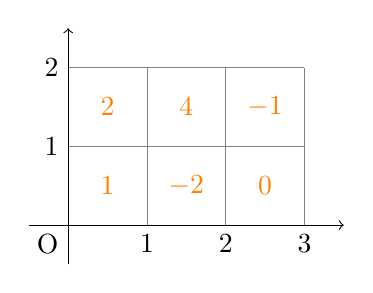
\begin{tikzpicture}
\draw[help lines,step=1] (0,0) grid (3,2);
\node[anchor=north east] at (0,0) {O};
\foreach \x in {1,2,3}
 \node[anchor=north] at (\x,0) {\x};
\foreach \y in {1,2}
 \node[anchor=east] at (0,\y) {\y};
 
\draw[->] (-0.5,0) -- (3.5,0);
\draw[->] (0,-0.5) -- (0,2.5);
\node[color=orange] at (0.5,0.5) {$1$};
\node[color=orange] at (1.5,0.5) {$-2$};
\node[color=orange] at (2.5,0.5) {$0$};
\node[color=orange] at (0.5,1.5) {$2$};
\node[color=orange] at (1.5,1.5) {$4$};
\node[color=orange] at (2.5,1.5) {$-1$};

\end{tikzpicture}

Total amount: \boxed{$4$}
\end{center}

If we refine the grid (let the number of grid squares go to infinity), we can consider this problem for a function $f(x,y)$, for example $f(x,y)=2x+y^2$. If this is the density on $U$, what is the amount now? 

\begin{center}
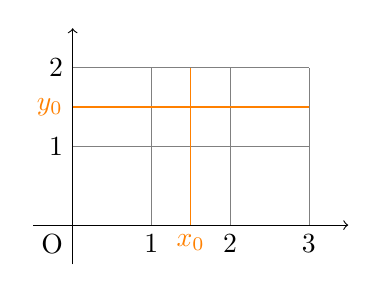
\begin{tikzpicture}
\draw[help lines,step=1] (0,0) grid (3,2);
\node[anchor=north east] at (0,0) {O};
\foreach \x in {1,2,3}
 \node[anchor=north] at (\x,0) {\x};
\foreach \y in {1,2}
 \node[anchor=east] at (0,\y) {\y};
 
\draw[->] (-0.5,0) -- (3.5,0);
\draw[->] (0,-0.5) -- (0,2.5);
\draw[-,color=orange] (1.5,0) -- (1.5,2);
\node[anchor=north,color=orange] at (1.5,0) {$x_0$};
\draw[-,color=orange] (0,1.5) -- (3,1.5);
\node[anchor=east,color=orange] at (0,1.5) {$y_0$};
\end{tikzpicture}
\end{center}
Let us, for example, hold the $x$-value constant at $x=x_0$. With the $x$-value held constant, we have now a function $h(y)=f(x_0,y)=2x_0+y^2$. We can then calculate the "total amount" on the vertical segment from $(x_0,0)$ to $(x_0,2)$. 
\begin{align*}
	&\hphantom{=}\int_0^2 f(x_0,y) dy \\
	&= \int_0^2 2x_0 + y^2 dy \\
	&= 2x_0y+\frac{1}{3}y^3 \Bigr\rvert_0^2 \\
	&= 4x_0+\frac{8}{3}
\end{align*}

Finally, the total amount over $U$ is obtained by integrating over the remaining $x$-variable: 
\[\int_{x=3}^3 4x_0 + \frac{8}{3} dx_0 = 2x_0^2 + \frac{8}{3} x_0 \Bigr\rvert_0^3=18+\frac{8}{3}3=26\]

This should be the same result as when we "go horizontally" first: 
\[\int_{y=0}^2\left(\int_{x=0}^32x+y^2 dx\right)dy=\int_{0}^2\left(x^2+xy^2\Bigr\rvert_0^3\right)dy=\int_0^2 9+3y\ dy=9y+y^3 \Bigr\rvert_0^2 =18+8=26\]

Intuitively, the following \ul{should} make sense: 
\begin{align*}
	\int_{[a,b]\times[c,d]} f(x,y) \left| d^2(x,y)\right| &=\int_a^b\System{\int_c^d f(x,y) dy}dx \\
	&=\int_c^d\System{\int_a^b f(x,y) dx}dy
\end{align*}
This (as well as its higher-dimensional analogs) is called \ul{Fubini's Theorem}. 

We can use these ideas without much complication to consider other types of regions:
\[\frac{x}{3}+\frac{y}{2}=1\]
\begin{center}
	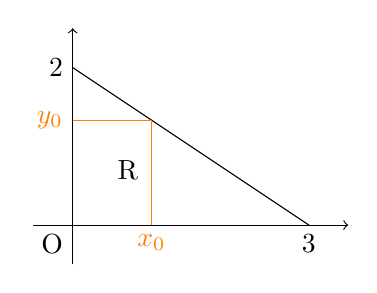
\begin{tikzpicture}
\node[anchor=north east] at (0,0) {O};
\foreach \x in {3}
 \node[anchor=north] at (\x,0) {\x};
\foreach \y in {2}
 \node[anchor=east] at (0,\y) {\y};
 
\draw[->] (-0.5,0) -- (3.5,0);
\draw[->] (0,-0.5) -- (0,2.5);
\draw[-] (0,2) -- (3,0);
\node[] at (0.7,0.7) {R};
\draw[-,color=orange] (1,4/3) -- (1,0);
\node[anchor=north,color=orange] at (1,0) {$x_0$};
\draw[-,color=orange] (0,4/3) -- (1,4/3);
\node[anchor=east,color=orange] at (0,4/3) {$y_0$};
\end{tikzpicture}
\end{center}
\[\int_R 2x+y^2 d^2(x,y) = \int_{x=0}^3\left(\int_{y=0}^{y=-\frac{2}{3}x+2}2x+y^2\ dy\right)\]

\end{document}